\documentclass[tikz, border=5mm]{standalone}

\usepackage{amsmath, amssymb, standalone}
\usetikzlibrary{arrows.meta, positioning, patterns, matrix}
\usetikzlibrary{decorations.pathreplacing}
\tikzstyle{box} = [rectangle, rounded corners, 
minimum width=2.5cm, 
minimum height=1cm,
align=center, 
draw=black, 
fill=blue!30]
\tikzstyle{arrow} = [->,thick]


\begin{document}
	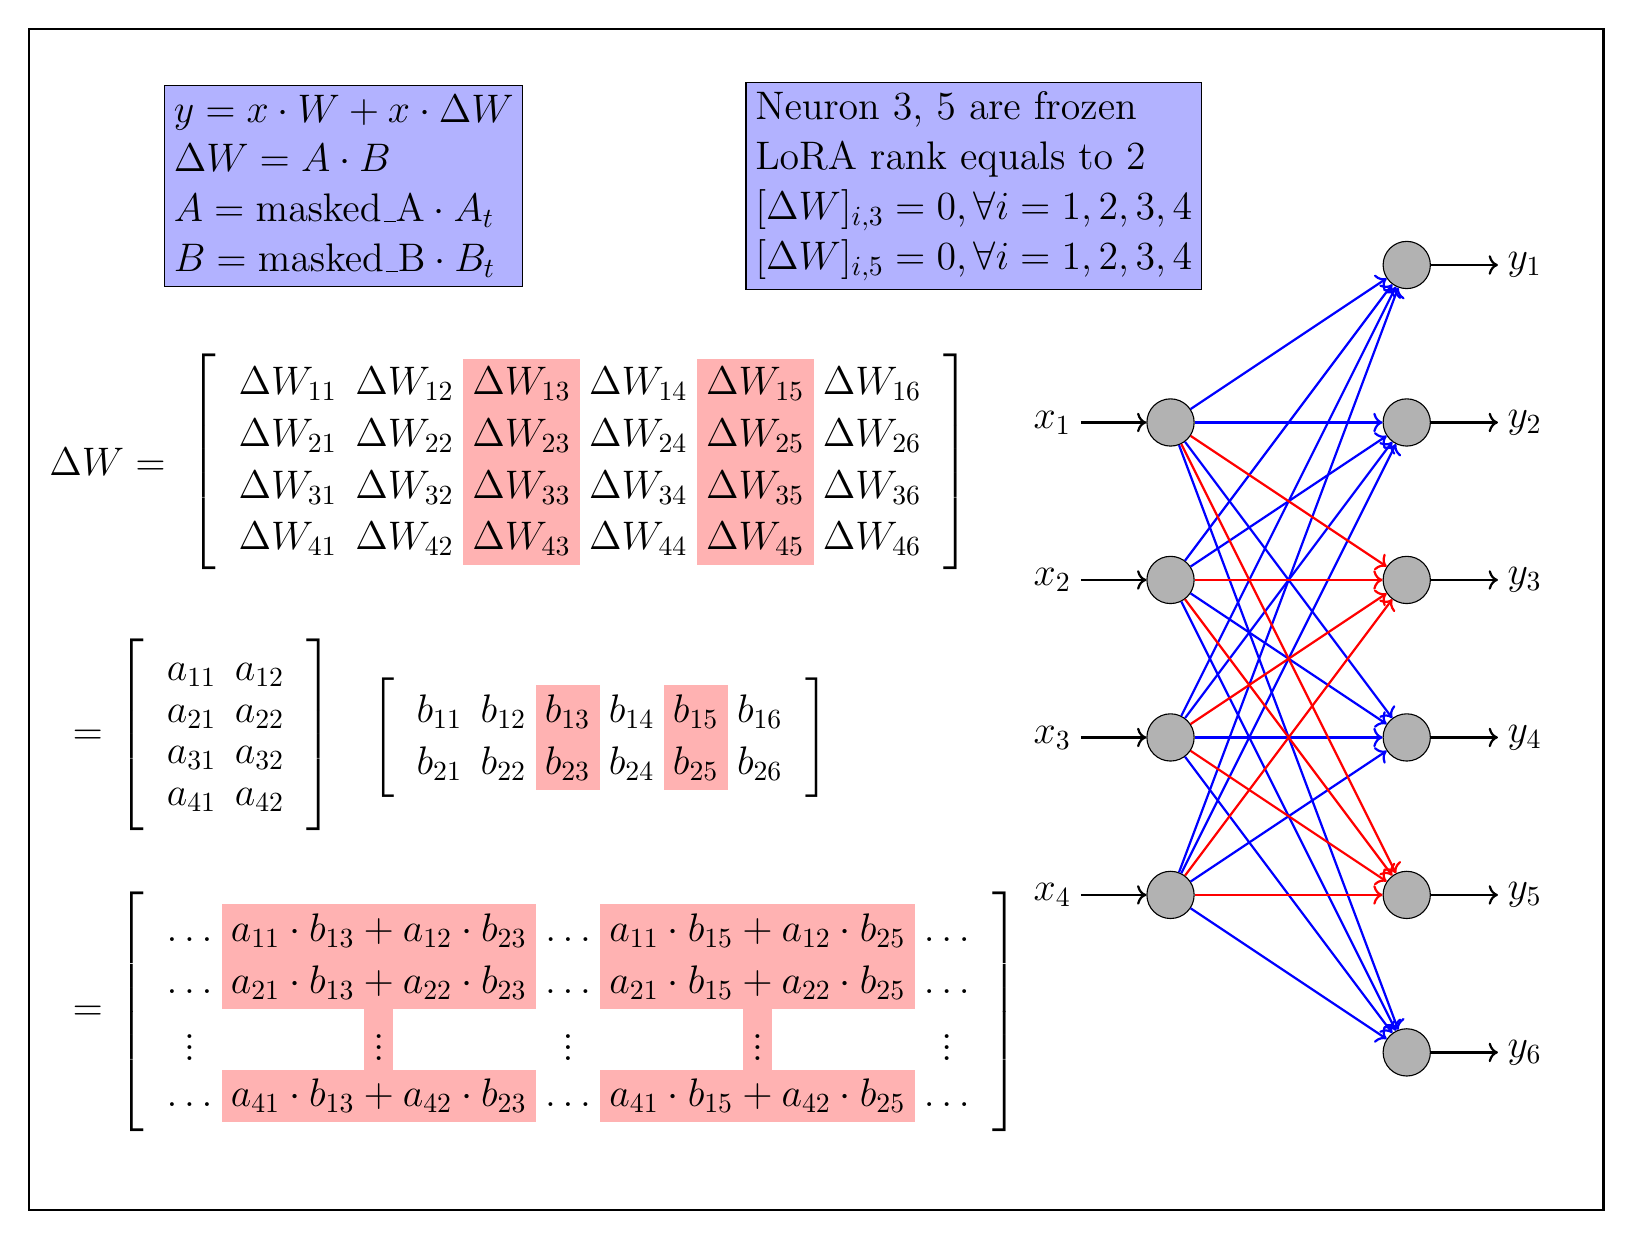
\begin{tikzpicture} [every node/.style={font=\Large}]
		
		% Define the canvas boundary (optional, for visualization)
		\draw[thick, black] (0,0) rectangle (20,15);
%		\draw[step=1cm,gray,very thin] (0,0) grid (20,20);
		
		% Input layer nodes
		\foreach \i in {1,2,3,4}
			\node (x\i) at (13, 12-2*\i) {$x_\i$};
		
		% Hidden layer nodes
		\foreach \i in {1,2,3,4}
			\node[circle, draw, minimum size=0.6cm, fill=black!30] (h\i) at (14.5, 12-2*\i) {};
	
		% Hidden layer nodes
		\foreach \i in {1,2,3,4,5,6}
			\node[circle, draw, minimum size=0.6cm, fill=black!30] (z\i) at (17.5, 14-2*\i) {};
		
		% Output layer nodes
		\foreach \i in {1,2,3,4,5,6}
			\node (y\i) at (19, 14-2*\i) {$y_\i$};
		
		% Draw connections (input to hidden)
		\foreach \i in {1,2,3,4}
			\draw[->, thick] (x\i) -- (h\i);
		\foreach \i in {1,2,3,4,5,6}
			\draw[->, thick] (z\i) -- (y\i);
		\foreach \i in {1,2,3,4}
			\foreach \j in {1,2,4,6}
				\draw[->, thick, blue] (h\i) -- (z\j);
		\foreach \i in {1,2,3,4}
			\foreach \j in {3,5}
				\draw[->, thick, red] (h\i) -- (z\j);
		
		\node[draw, align=left, font=\Large, fill=blue!30] (equations) at (4,13) {
			$y = x \cdot W + x \cdot \Delta W$ \\
			$\Delta W = A \cdot B$ \\
			$A = \text{masked\_A} \cdot A_{t}$ \\
			$B = \text{masked\_B} \cdot B_{t}$
		};
		\node[draw, align=left, font=\Large, fill=blue!30] (textbox) at (12, 13) {
			Neuron 3, 5 are frozen \\
			LoRA rank equals to 2 \\
			$[\Delta W]_{i, 3} = 0, \forall i = {1, 2, 3, 4}$ \\
			$[\Delta W]_{i, 5} = 0, \forall i = {1, 2, 3, 4}$ 
			
		};
		
		% Delta W matrix (4 by 6)
		\node at (1, 9.5) {\( \Delta W = \)};
		\node (deltaW) [matrix of math nodes, nodes in empty cells, left delimiter={[}, right delimiter={]}, column 3/.style={nodes={fill=red!30}}, column 5/.style={nodes={fill=red!30}}] at (7, 9.5) {
			\Delta W_{11} & \Delta W_{12} & \Delta W_{13} & \Delta W_{14} & \Delta W_{15} & \Delta W_{16} \\
			\Delta W_{21} & \Delta W_{22} & \Delta W_{23} & \Delta W_{24} & \Delta W_{25} & \Delta W_{26} \\
			\Delta W_{31} & \Delta W_{32} & \Delta W_{33} & \Delta W_{34} & \Delta W_{35} & \Delta W_{36} \\
			\Delta W_{41} & \Delta W_{42} & \Delta W_{43} & \Delta W_{44} & \Delta W_{45} & \Delta W_{46} \\
		};
		
		% Define the first matrix
		\node at (0.75, 6) {\( = \)};
		\node (matrixA) [matrix of math nodes,left delimiter={[},right delimiter={]},nodes in empty cells] at (2.5, 6) {
			a_{11} & a_{12} \\
			a_{21} & a_{22} \\
			a_{31} & a_{32} \\
			a_{41} & a_{42} \\
		};
		
		% Define the second matrix
		\node (matrixB) [matrix of math nodes,left delimiter={[},right delimiter={]},nodes in empty cells, column 3/.style={nodes={fill=red!30}}, column 5/.style={nodes={fill=red!30}}] at (7.25, 6) {
			b_{11} & b_{12} & b_{13} & b_{14} & b_{15} & b_{16} \\
			b_{21} & b_{22} & b_{23} & b_{24} & b_{25} & b_{26} \\
		};
		
		% Define the result matrix
		\node at (0.75, 2.5) {\( = \)};
		\node (matrixC) [matrix of math nodes,left delimiter={[},right delimiter={]},nodes in empty cells, column 2/.style={nodes={fill=red!30}}, column 4/.style={nodes={fill=red!30}}] at (6.85, 2.5) {
			\dots & a_{11} \cdot b_{13} + a_{12} \cdot b_{23} & \dots & a_{11} \cdot b_{15} + a_{12} \cdot b_{25} & \dots\\
			\dots &  a_{21} \cdot b_{13} + a_{22} \cdot b_{23} & \dots & a_{21} \cdot b_{15} + a_{22} \cdot b_{25}  & \dots\\
			\vdots & \vdots & \vdots & \vdots & \vdots \\
			\dots &  a_{41} \cdot b_{13} + a_{42} \cdot b_{23}  & \dots & a_{41} \cdot b_{15} + a_{42} \cdot b_{25}  & \dots\\
		};

		
	\end{tikzpicture}
	
\end{document}